\documentclass{article}
\usepackage[catalan]{babel}
\usepackage{graphicx}
\usepackage{moresize}
\usepackage{amssymb}
\usepackage{caption}
\usepackage{subcaption}
\usepackage{amsmath}
\usepackage{wrapfig}
\usepackage{xcolor}
\usepackage{mathtools}
\usepackage{esint}
\usepackage{siunitx-v2}
\usepackage{epstopdf}
\usepackage{mhchem}
\usepackage{colortbl}
\usepackage{multirow}
\usepackage{hyperref}
\usepackage[labelfont=bf, font=footnotesize, textfont=sl, skip=3pt, width=0.95\textwidth]{caption}
\hypersetup{
	colorlinks=true,
	linkcolor=black,
	filecolor=white,      
	urlcolor=cyan,
	pdftitle={Overleaf Example},
	pdfpagemode=FullScreen,
}
\usepackage{mathrsfs}
\usepackage{graphicx}
\usepackage{imakeidx}
\usepackage{fancyhdr}
\usepackage[a4paper, total={6in, 9in}]{geometry}
\pagestyle{fancy}
\lhead[Universitat Autònoma de Barcelona]{Universitat Autònoma de Barcelona}
\rhead[Termodinàmica i Mecànica Estadística]{Termodinàmica i Mecànica Estadística}
\newcommand*{\mybox}[1]{\framebox{#1}}

\thispagestyle{empty}

\begin{document}
	
	\begin{titlepage}
		\begin{center}
			\vspace*{1cm}
			
			\Huge
			\textbf{Treball de Simulació} \\
			Gas d'esferes dures
			
			\vspace{0.5cm}
			
			
			
			
			\vspace{1.5cm}
			\Large
			Àxel Cortés; 1566285 \\
			Joan Vidal Escobosa; 1667487 \\
			Jan Franco; 1628517 \\ 
			
			
			\vfill
			\LARGE
			
			\vspace{0.8cm}
			
			\Large
			Curs 2024-25 
		\end{center} 
	\end{titlepage}
	
	\setcounter{page}{1}
	
	
	\section{Gas d'esferes dures. Temps entre col·lisions, pressió experimental i cicle d'Stirling}
	
	
	En aquesta primera secció donem resposta a les qüestions 1 i 2 del treball. Partim d'un codi que ens simula un conjunt d'esferes dures limitades per les parets d'una caixa cúbica. Les partícules van xocant amb les parets de la caixa i entre elles. El primer que cal fer és veure com és el temps mig de col·lisió (mitjana de la diferència de temps que hi ha entre una col·lisió i la següent) per comparar-lo amb el teòric. Podem veure una imatge de la simulació que ens proporciona el codi així com del gràfic de distribució de velocitats que inclou (figura \ref{gugugu}.) \\
	
	
	\begin{figure}[h!]
		\centering
		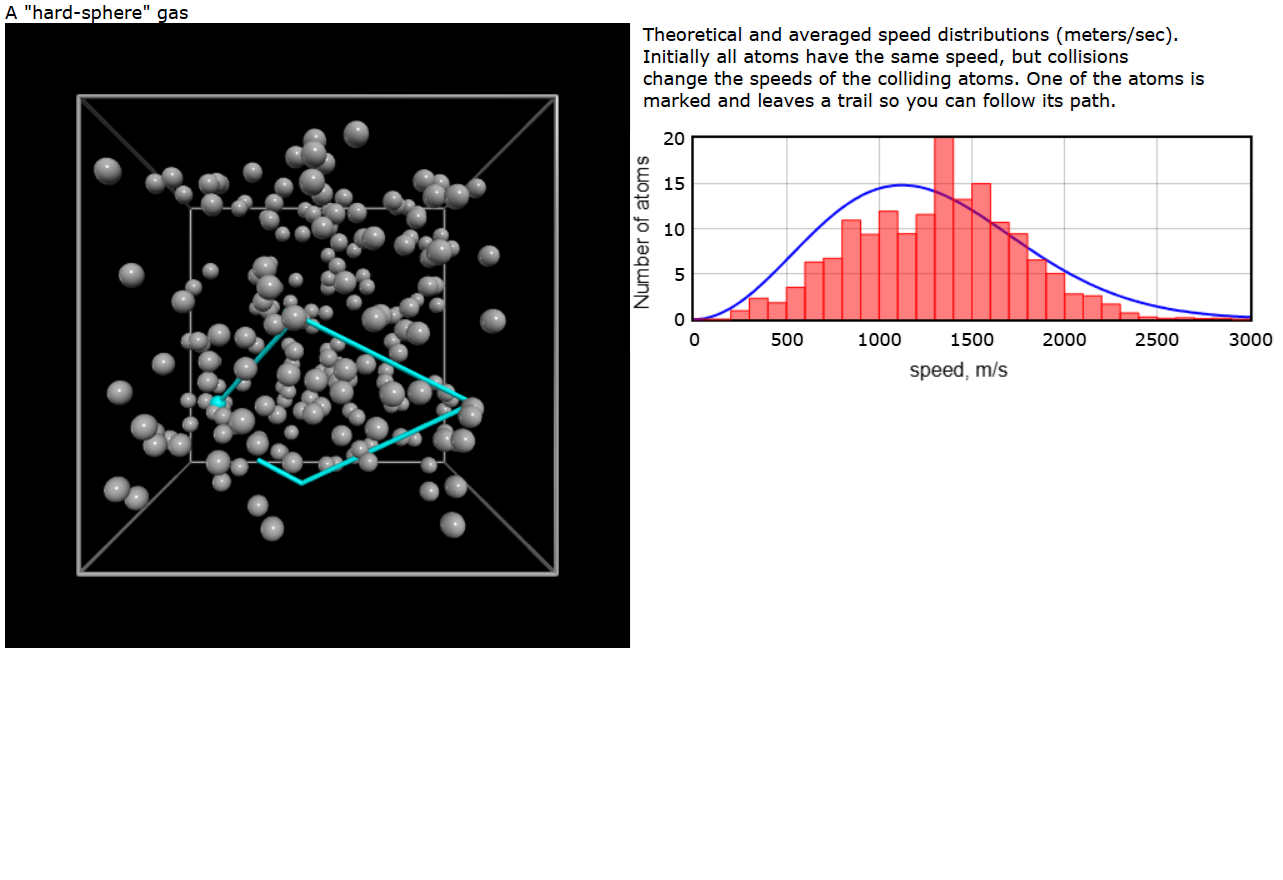
\includegraphics[width=0.7\linewidth]{Interfaç.png}
		\caption{Evolució de $C_V$ en funció del nombre d'iteracions realitzades, utilitzant utilitzant $10^4$ partícules, fent $10^7$ iteracions i a una T = 300 K}
		\label{gugugu}
	\end{figure}
	
	\subsection*{Q1}

	El primer que cal és buscar una expressió que ens calculi el temps mig entre col·lisions a partir de les condicions del sistema. Per a lograr això buscarem primer la freqüència entre col·lisions, $Z_{col}$. Aquesta dependrà de la freqüència d'àtoms que passin per una regió de l'espai amb la mida d'un àtom. Tenim, doncs:
	$$
	\begin{aligned}
		Z_i & =\frac{\sqrt{2} \pi d^2\langle v_r\rangle \Delta t\left(\frac{N}{V}\right)}{\Delta t} \\
		Z_i & =\sqrt{2} \pi d^2\langle v_r\rangle\left(\frac{N}{V}\right)
	\end{aligned}
	$$
	On $\langle v_r \rangle = \sqrt{\frac{8k_BT}{\pi m}}$ és la velocitat mitja que porten les partícules, i es pot deduir a partir de la distribució Maxwell-Boltzmann. $N$ i $V$ són el nombre d'àtoms i el volum total; i $d$ és la distància màxima en la que es troben dos àtoms que acaben xocant (i segeuixen una trajectoria recta). Si volem calcular la freqüència total cal considerar la densitat de partícules al recipient, no només la freqüència de xoc.
	$$
	\begin{gathered}
		Z_{\text{col}}=\frac{1}{2} Z_i\left(\frac{N}{V}\right) \\
		Z_{\text{col}}=\frac{\sqrt{2}}{2} \pi d^2\langle c\rangle\left(\frac{N}{V}\right)^2
	\end{gathered}
	$$
	Com a velocitat mitja trobem un valor de $\boxed{\langle v_r \rangle = 1257.84}$. Usant $d=R_{\text{àtom}} = 0.03$, $N=500$ i $V=1$ m$^3$ trobem un valor teòric del temps mig entre col·lisions de: 
	\begin{equation}
		\boxed{T_{\text{col}}^{\text{TEO}} = \frac{1}{Z_{\text{col}}} = 3.9765 \cdot 10^{-7}}
	\end{equation}
	
	
	
	\par Per a la part experimental procedirem com hem dit a l'inici, fent ús del codi ja proporcionat sobre un gas d'esferes dures. D'aquesta manera, només ens cal variar el nombre d'àtoms (el fixem a 500) i afegir una llista que conservi tots els temps entre col·lisions, després fem la mitjana d'aquests valors i ho comparem amb el teòric. Una bona manera és anar enregistrant el temps i contant les col·lisions; per tenir el temps mig només cal anar dividint intervals de temps entre el nombre de col·lisions que s'hi donen. El valor obtingut experimentalment és: 
	\begin{equation}
		\boxed{\langle T_{\text{col}}\rangle = 2.294762 \cdot 10^{-7}}
	\end{equation}
	 
	Com veiem el resultat difereix menys d'un ordre de magnitud del supòsit teòric, pel que el prenem per bo. Tot i això veiem que tenim un error del $42.3\%$. Cal tenir en compte que el resultat teòric realitza unes quantes aproximacions que potser no compleix un gas on es suposa que els àtoms d'heli mesuren $3$ centímetres de radi. 
	
	
	\subsection*{Q2}
	
	
	
	\subsection*{Q3}
	Per tal d'implementar el procés isoterm, s'ha modificat el codi de manera que s'ha simulat un termostat encarregat de reiniciar l'energia cinètica de les partícules a cada interval de temps per mantenir la temperatura constant. Utilitzant el mètode de Verlet, podem simular el moviment d'una de les parets per tal de comprimir el gas d'esferes dures. A la simulació hem afegit un gràfic de la variació del producte de la pressió i el volum. Segons la llei dels gasos ideals aquest producte no ha de variar si tenim el sistema a temperatura i nombre de mols constants. Ens assegurem de que el procès sigui quasiestàtic donant valors petits de diferencials de temps. Podem veure el resultat de l'experiment a la gràfica \ref{cacafuti}
	
	\begin{figure}[h!]
		\centering
		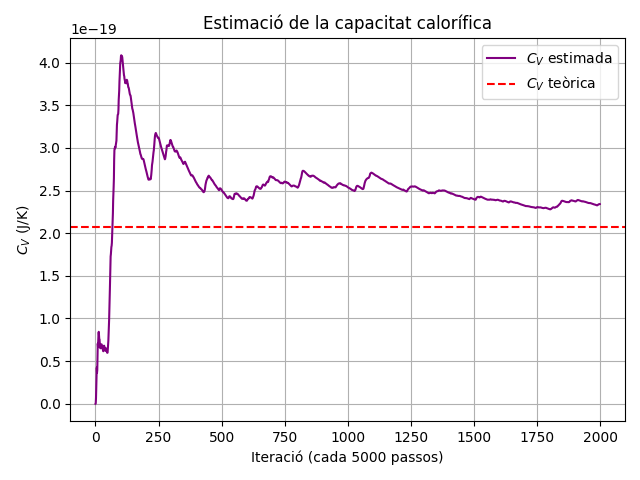
\includegraphics[width=0.7\linewidth]{MonteCarlo.png}
		\caption{Representació del producte pressió per volum front el temps. Corroborem un comportament constant del sistema.}
		\label{cacafuti}
	\end{figure}
	
	Com es veu de la figura de just a sobre tenim un resultat de $PV$ quasi-constant en el temps. Tot i això, el gràfic té uns pics molt pronunciats que semblen trencar amb el supòsit que es comportaria com un gas ideal. Cal veure el que realment està passant: nosaltres només podem suposar un termostat si atribuïm una energia cinètica constant a les partícules. Com que aquestes van xocant entre elles cal anar donant uns valors dins d'un rang determinat i fer que totes les molècules que es mantinguin en aquest rang (és a dir, anar deliberadament modificant el moment lineal de les partícules per a que no varii). Si just el programa agafa un valor de $PV$ on el temrostat encara no ha actuat sobre les molècules de sobte surt un valor diferent ja que la temperatura és diferent. Com que ràpidament torna a la temperatura que hem fixat el valor torna al constant de $PV$ i en el gràfic apareix un pic. Podriem solucionar aquest inconvenient donant uns intervals de temps més petits.
	
	
	
	\subsection*{Q4}
	Un procés de Stirling consta de dos processos isocòrics i dos processos isotèrmics, com veiem en la figura \ref{gurururur}.
	Com ja hem vist a la qüestió anterior, podem simular computacionalment un termostat i un èmbol mòbil que expandeix el gas a temperatures altes. Similarment, per l'altre procés isotèrmic, es comprimeix el gas a una temperatura més baixa però la simulació es essencialment la mateixa. Consta d'un termostat que reinicia la energia cinètica de les esferes dures per simular una constància en la temperatura i un èmbol mòbil que representi el canvi de volum.\\
	\begin{figure}[h!]
		\centering
		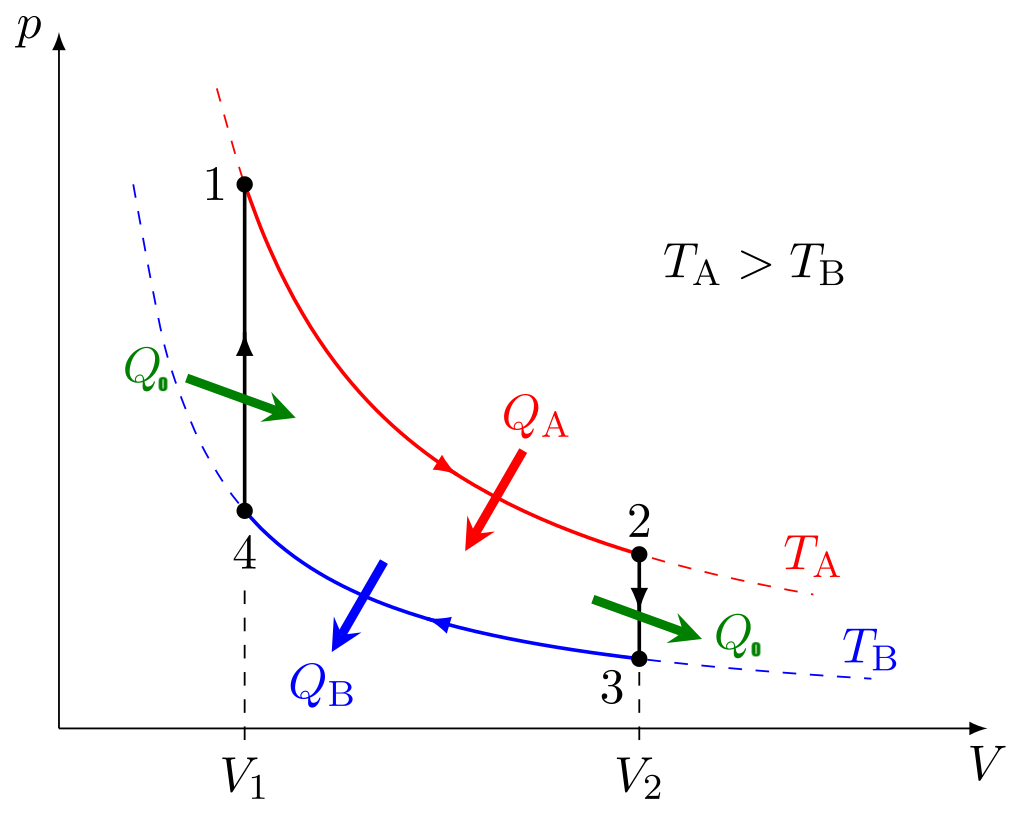
\includegraphics[width=0.5\linewidth]{Ciclo_de_Stirling_pV.png}
		\caption{}
		\label{gurururur}
	\end{figure}	
	
	

	
	\par D'aquesta manera hauriem de simular com el l'exercici dos els processos $1\to 4$ i $2 \to 3$; i hauriem de simular com en l'exercici tres els processos $1\to2$ i $3\to4$. Per trobar el rendiments només ens cal comparar la calor que surt en funció de la que entra (la $Q_0$ és una calor en teoria constant, que no va donant ni fent pedre calor al sistema al llarg d'un cicle). Per a lograr això operem de la següent manera: 
	$$
	\eta =\frac{Q_A - Q_B}{Q_A}=\frac{W}{Q_A}
	$$
	Per a trobar $W$, o sigui, el treball que fa la màquina només ens cal usar els resultats d'estructura de la termodinàmica.  Tenim: $W = \int_{V_1}^{V_2} pdV$. Computacionalment es pot trobar fent el càlcul $V_{i}-V_{i-1}$ on $i$ marca l'índex d'un bucle de molts passos, com més millor. Els valors del volum per a cada punt els podem calcular amb la llei dels gasos i multiplicant per el valor $p_{i}$ i sumant tots els resultats tindrem $W$. Finalment el podem comparar amb el cas ideal en el qual el motor és una màquina de Carnot. En aquestes circumstàncies el rendiment serà: 
	$$
	\eta = 1- \frac{T_B}{T_A}
	$$ 
	\section{Fuid de Lennard-Jones}
	
	\subsection*{Q5}
	
	Volem estudiar doncs la coexistència de fases líquides i gasoses al voltant de la temperatura crítica ($T_c$). Recuperant que les densitats depenen de la temperatura;
	\begin{equation} \label{bambi}
		\rho_l-\rho_g = A\left( 1-\frac{T}{T_C}\right)^\beta
	\end{equation}
	Podem utilitzar la simulació que permet veure l'equilibri de fases per observar el valor de la temperatura crítica. 
	Per tal de trobar aquest valor hem de tenir dos consideracions en compte degut a les propietats del punt crític. En les condicions analitzades les fases es fan indistingibles i per tant els volums específics s'igualaran.
	En conseqüència, les densitats també ja que $(v=\frac{1}{\rho})$.
	Per altra banda, a prop del punt crític;
	\begin{equation}
		\frac{\partial T}{\partial \rho}=0
	\end{equation}
	És a dir, trobant el màxim que ens proporciona la gràfica densitat-temperatura de la simulació aconseguim el valor de la temperatura crítica.
	Trobem doncs que la temperatura crítica és de
	\boxed{T_c=1.32K}.
	\\
	\\
	
	Per l'estudi dels paràmetres $\beta$ i A estudiem diferents temperatures i acomodant l'expressió \ref{bambi} fem una regressió lineal (veure figura \ref{1}.
	
	\begin{equation}
		\ln(\rho_l-\rho_g)=\beta \ln\left(1-\frac{T}{T_c}\right)+ \ln A
	\end{equation}
	Amb el que obtenim valors de
	\\
	\boxed{\beta=0,324\pm 0,013} i \boxed{A=1,041\pm0,021}
	
	Consultant el valor tabulat de $\beta$ trobem que el valor teòric $\beta=0,32$ es compatible amb el nostre resultat.
	\begin{figure}[h!] 
		\centering
		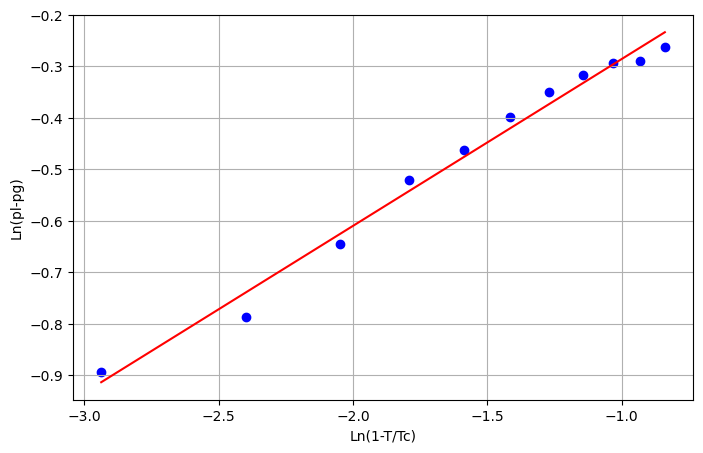
\includegraphics[width=0.7\linewidth]{regresionq5.png}
		\caption{Regressió lineal dels valors experimentals}
		\label{1}
	\end{figure}
	
	
	
	\section{Creació d'una simulació de Monte Carlo pròpia}
	\subsection*{Q6, 7, 8}
	En aquest apartat hem generat un codi, que podem trobar a l'Annex, que simula un gas ideal en col·lectivitat canònica de d dimensions (d = 1,2,3) amb tècniques de Monte Carlo.
	\\
	El codi inicialitza velocitats de partícules segons una distribució de Maxwell-Boltzmann. A cada pas, tria una partícula aleatòriament i proposa un petit canvi en la seva velocitat. Després, decideix si acceptar aquest canvi segons el criteri de Metropolis, el qual accepta tots els canvis energèticament favorables i els energèticament desfavorables amb una probabilitat de $e^{\frac{-\Delta E}{k_BT}}$. Per últim, cada 500 passos mesura l'energia total del sistema per a poder-ne trobar la capacitat calorífica.
	\\
	Aquesta la podem trobar amb la següent fórmula:
	
	\begin{equation}
		C_V = \frac{\langle E^2 \rangle - \langle E \rangle^2}{k_B T^2}
		\label{eq. c_v}
	\end{equation}
	
	\noindent L'energia mitjana del sistema i el valor mitjà del seu quadrat són, respectivament:
	
	\begin{gather}
		\langle E \rangle = \sum_i E_i \cdot P(E_i)
		= \frac{1}{Z} \sum_i E_i e^{-E_i / (k_B T)}
		\\
		\langle E^2 \rangle = \sum_i E_i^2 \cdot P(E_i)
		= \frac{1}{Z} \sum_i E_i^2 e^{-E_i / (k_B T)}
	\end{gather}
	
	\noindent Considerant el sistema en el límit termodinàmic, ($\langle E \rangle  \, = \, U$) i tenint en compte que la capacitat calorífica a volum constant es defineix com:
	
	\begin{equation}
		C_V = \left( \frac{\partial \langle E \rangle}{\partial T} \right)_V
	\end{equation}
	
	\noindent Podem realitzar aquesta derivada per acabar arribant a l'Eq. \eqref{eq. c_v}.
	\\
	Fixem-nos, per tant, que les fluctuacions d'energia estan directament relacionades amb la capacitat calorífica del sistema.
	\\
	
	\noindent Hem fet córrer la simulació diverses vegades, i utilitzant els valors de $10^4$ partícules, fent $5 \cdot 10^6$ iteracions i una $T =  300 \, K$, no hem obtingut en cap cas una diferència major al $15 \, \%$ entre els valors de $C_V$ simulats i els teòrics, donats per $C_V = \frac{d}{2}Nk_B$. La Taula \ref{taula_comparacio} mostra un exemple per cada dimensió de valors obtinguts en la simulació.
	
	\begin{table}[h!]
		\centering
		\begin{tabular}{|c|c|c|c|}
			\hline
			\textbf{Dimensió} & \textbf{$C_V$ teòrica (J/K)} & \textbf{$C_V$ simulada (J/K)} & \textbf{Diferència relativa (\%)} \\ \hline
			1 & $6.900 \times 10^{-20}$ & $6.188 \times 10^{-20}$ & 10.316 \\ \hline
			2 & $1.380 \times 10^{-19}$ & $1.252 \times 10^{-19}$ & 9.299 \\ \hline
			3 & $2.070 \times 10^{-19}$ & $2.208 \times 10^{-19}$ & 6.665 \\ \hline
		\end{tabular}
		\caption{Exemples de capacitats calorífiques simulades i valors teòrics per a d=1,2 i 3 utilitzant $10^4$ partícules, fent $5 \cdot 10^6$ iteracions i a una T = 300 K}
		\label{taula_comparacio}
	\end{table}
	
	Per últim, hem graficat a la Figura \ref{figura_evolucio_C_V}  com evoluciona el valor calculat de $C_V$, per d=3, en funció del nombre d'iteracions realitzades, per veure si aquest acaba estabilitzant-se. Veiem que el valor oscil·la en un rang reduït de valors, pel que la seva diferència respecte al valor teòric no és deguda a que es necessitin més iteracions. De fet, si volguéssim més precisió hauríem d'augmentar el nombre de partícules, acostant-nos més així al límit termodinàmic que hem considerat en els nostres càlculs. 
	
\begin{figure}
	\centering
	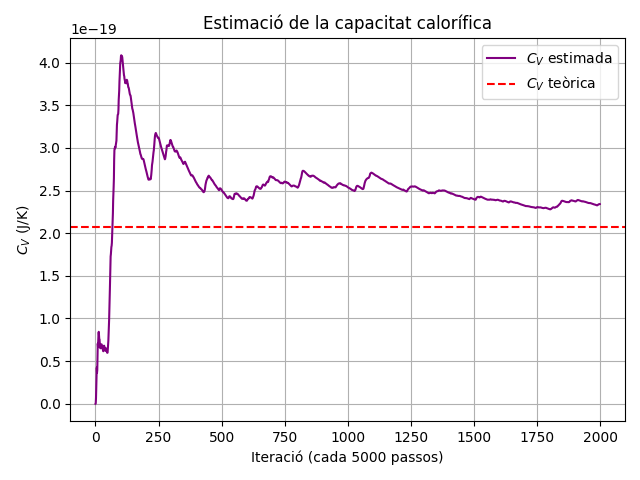
\includegraphics[width=0.7\linewidth]{MonteCarlo.png}
	\caption{Evolució de $C_V$ en funció del nombre d'iteracions realitzades, utilitzant utilitzant $10^4$ partícules, fent $10^7$ iteracions i a una T = 300 K}
	\label{figura_evolucio_C_V}
\end{figure}
	
	
\end{document}